\chapter{Статический контроль \\ за изменяемостью объектов}

\section{Подход к технической реализации}

Предположим, нужно добавить некоторую новую функциональность в язык программирования. Есть два принципиально разных способа это сделать:
\begin{itemize}
	\item использовать существующие средства языка
	\item изменять синтаксис языка (например, добавить новые ключевые слова)
\end{itemize}

У обоих этих подходов есть как положительные, так и отрицательные стороны. Изменение синтаксиса языка приводит к невозможности использования многих существующих инструментов для разработки с использованием этого языка, таких как компиляторы, среды разработки, различные анализаторы кода. Но с другой стороны этот подход позволяет добавлять в язык развитую систему выразительных средств. Использование же существующих средств языка ограничивает свободу введения новых концепций, но этот подход обычно гораздо проще в реализации и не влияет на используемые инструменты.

В случае Java есть несколько способов добавить поддержку неизменяемости объектов в язык. В работе IGJ это сделано с помощью добавления дополнительного типового параметра ко всем классам. Но это выглядит очень громоздко и трудно читаемо. Другой варинат -- использование аннотаций. 

Аннотация в Java -- это вид метаданных, которые могут быть добавлены в исходный код. Они могут быть доступны на этапе компилляции, в класс-файлах, а также могут использоваться JVM во время исполнения программы. В Java 7 аннотации можно применять к пакетам, классам, методам, переменным и параметрам. 

Как справедливо отмечают некоторые авторы, аннотации в том виде, в котором они реализованы в Java 7, не достаточно мощны для того, чтобы добавить поддержку контроля за изменяемостью объектов, так как в нынешней реализации нельзя аннотировать типы. Но уже в Java 8 такая поддержка появится, поэтому в данной работе именно аннотации используются для выражения неизменяемости объектов.

\section{Система аннотаций}

Будем считать, что каждая ссылка имеет модификатор изменяемости, который определяет, может ли быть изменено абстрактное состояние объекта, на который она ссылается. Этот моификатор определяется на уровне исходного кода, анализуруется на этапе компиляции и может иметь одно из четырех значений: @Mutable, @Immutable, @ReadOnly или @Isolated. На изображении ниже представлена иерархия параметров неизменяемости. 

\begin{figure}[h]
\center{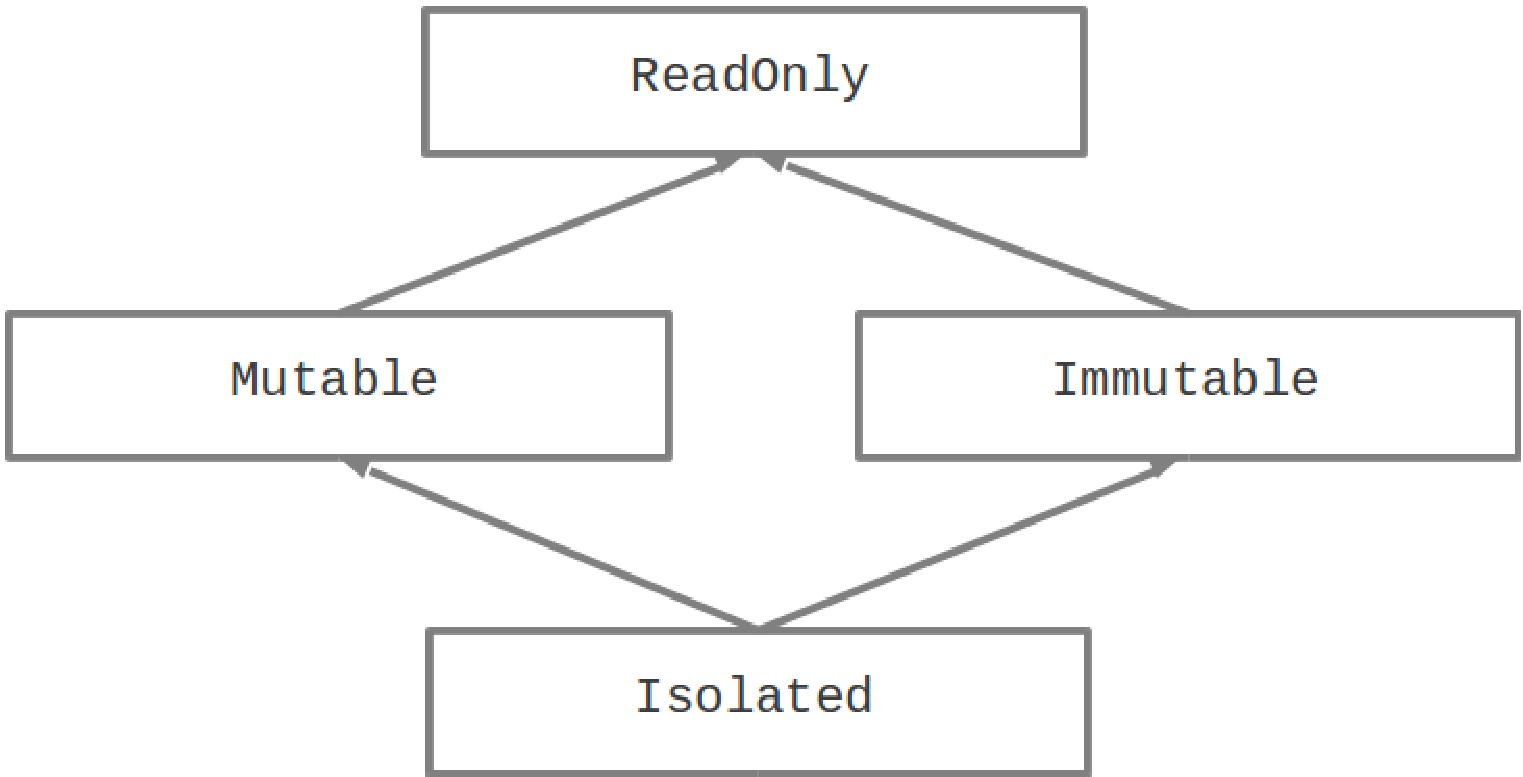
\includegraphics[scale=0.4]{my_classes.pdf}}
\caption{Иерархия модификаторов неизменяемости}
\label{pic:my_classes}
\end{figure}

Выражение $A \preceq B$ будем тракторвать как "$A$ является наследником $В$". В данном случае, например, $Mutable \preceq ReadOnly$. Также будем считать, что если $A \preceq B$, где $А$ и $B$ - модификаторы изменяемости, то $@A\:C \preceq @B\:C$, где $С$ - некий тип.

\subsection{Ссылочная неизменяемость}

Для поддержки ссылочной неизменяемости достаточно двух модификаторов: @Mutable и @ReadOnly. Состояние объекта не может быть изменено через @ReadOnly ссылку. Попытка присвоить поле через @ReadOnly ссылку или вызвать на ней меняющий объект метод приведет к ошибке компиляции:

\begin{lstlisting}[caption=Mutable и RadOnly ссылки, label=code:mutable_vs_readonly]
@ReadOnly Person roPerson = ...;
String address = roPerson.address; // OK: reading field is 
                                   // always permitted
roPreson.address = "new address"; // Error: field can't be 
                       // assigned through ReadOnly referernce

@Mutable Person mPreson = ...;
mPerson.address = "new address"; // OK: mPerson is mutable, 
                                 // so field can be assigned
\end{lstlisting} 

Пусть I(x) - это функция, которая принимает класс, тип или ссылку и возвращает ее модификатор изменяемости. Тогда вышеизложенное правило может быть написано следующим образом:

\begin{Rule}\label{rule:assign_field}
o.someField = ... разрешено тогда и только тогда, когда $I(o) = Mutable$ 
\end{Rule}

Изменяемая ссылка может быть передана везде, где ожидается неизменяемая ссылка. Таким образом, @Mutable Person является наследником @ReadOnly Person.

\subsection{Аннотации на методах}

В Java ключевое слово this внутри конструктора или нестатического метода является ссылкой на текущий объект.  Изменяемость this зависит от контекста, а именно от метода, в котором появляется this. По умолчанию все методы изменяют объект, на котором вызываются. В таких методах this будет иметь модификатор @Mutable. Те методы, которые не изменяют объект, на котором они вызываются, должны быть помечены аннотацией @Const (по аналогии с C++), this в этих методах будет иметь модификатор @ReadOnly.

На @ReadOnly ссылках нельзя вызывать методы, которые меняют объект, на котором вызываются. Формально это правило может быть описано так:

\begin{Rule}\label{rule:invoke_method}
o.m(...) разрешено, если $I(o) \preceq I(m)$, где I(m) -- модификатор изменяемости this в этом методе.
\end{Rule}

Требуется, что $I(o) \preceq I(m)$ а не $I(o) = I(m)$ для того, чтобы через изменяемую ссылку можно было вызывать методы, не меняющие объект. 

Рассмотрим на примере применение этих правил.

\begin{lstlisting}[caption=Аннотации на методах, label=code:method_annotations]
class Person {
    String name;
    @AsClass Date dateOfBirth;	
    
    public Person(String name, Date dateOfBirth) {
    	this.name = name;
    	this.dateOfBirth = dateOfBirth;
    }
    
    public void setName(String name) {
        this.name = name;
    }
    
    @Const
    public String getName() {
        return name;
    }
    
    @AsClass
    @Const
    public Date getDateOfBirth() {
        return dateOfBirth;
    }
    
    @Const 
    public boolean wasBornInYear(int year) {
    	return dateOfBirth.getYear() == year;
    }
    
    public void setYearOfBirth(int year) {
        dateOfBirth.setYear(year);
    }
    
    public static void print(@ReadOnly Person person) {
        ...
    }
}
\end{lstlisting} 

Присваивание this.name = name в 11 строке разрешено, так как $I(this) = I(setName) = Mutable$, а согласно правилу \ref{rule:assign_field} через @Mutable ссылку можно присваивать значение поля. Это присваивание было бы не разрешено, если бы оно было перемещено  на 16 строку, так как this является @ReadOnly ссылкой в контексте метода getName. Вызов метода setYear на 31 строке разрешен согласно правилу \ref{rule:invoke_method}, так как $I(dateOfBirth) = I(this) \preceq I(setyearOfBirth)$. Этот вызов метода не был бы разрешен на 27 строке, так как в контексте метода wasBornInYear $I(this) = ReadOnly$. Статический метод print на 34 строке принимает объект класса Person с любым модификатором изменяемости. 

Поле dateOfBirth проаннотировано @AsClass. Это значит, что его модификатор изменяемости зависит от того, какой модификатор у this. Соответсвенно и результатом работы метода getDateOfBirth будет либо @Mutable ссылка (если сам он был вызван на объекте, доступном по @Mutable ссылке), либо @ReadOnly ссылка в противном случае:

\begin{lstlisting}[caption=Использование аннотации AsClass, label=code:as_class]
@ReadOnly Person roPerson = ...;
// OK: I(getYear) = ReadOnly
int year = roPerson.getDateOfBirth().getYear(); 
// OK: I(roPerson.getDateOfBirth()) = I(roPerson) = ReadOnly
roPerson.getDateOfBirth().setYear(2000); 
	
@Mutable Person mPerson = ...;
// OK: I(mPerson.getDateOfBirth()) = I(mPerson) = Mutable
mPerson.getDateOfBirth().setYear(2000); 
\end{lstlisting} 

Аннотация AsClass может встречаться на полях метода, локальных переменных, возвращаемых значениях нестатических методов и параметрах методов.

\subsection{Перегрузка методов}

При перегрузке методов, метод класса-потомка должен оставить прежним или усилить модификатор неизменяемости, который имеет this в данном методе. 

\begin{Rule}\label{rule:override_method}
Если метод $m'$ перегружет метод m, то $I(m) \preceq I(m')$
\end{Rule}

Например, метод класса-потомка может добавить аннотацию Const к перегружаемому методу, если ее не было в классе-предке, но не наоборот. 

\subsection{Объектная неизменяемость}

Хотя @ReadOnly ссылки запрещают менять объект, на который ссылаются, никто не гарантирует, что этот объект не будет изменен при помощи какой-либо другой ссылки. Это хорошо иллюстрирует слудющий пример:

\begin{lstlisting}[caption=Изменение объекта\, хранимого по @ReadOnly ссылке, label=code:change_ro_object]
@Mutable Person person = ...;
person.setYearOfBirth(2000);
@ReadOnly Person roPerson = person; // OK: @ReadOnly Person is 
                                    // supertype for 
                                    // @Mutable person
// 2000 will be printed
System.out.println(roPerson.getyearOfBirth());
person.setyearOfBirth(2013);
// 2013 will be printed
System.out.println(roPerson.getyearOfBirth()); 			
}
\end{lstlisting} 

При этом часто возникает ситуация, когда хочется не только гарантировать, что по данной ссылке нельзя менять объект, но и то, что данный объект вообще нельзя менять. Такие гарантии могут быть полезны, например, при многопоточном программировании -- если про объект известно, что он неизменяемый, то к нему можно безопасно обращаться из нескольких потоков без дополнительной синхронизации. Разработанная в данной работе система может давать такую гарантию: @Immutable ссылка всегда указывает на неизменяемый объект. 

\begin{lstlisting}[caption=@Mutable и @Immutable ссылки, label=code:mutable_vs_immutable]
@Mutable Person person = ...;
@Immutable Person iPerson = person; // Error: @Immutable Person is 
                                    // not supertype for 
                                    // @Mutable Person
@ReadOnly Person roPerson = iPerson; // OK: @ReadOnly Person is 
                                     // supertype for 
                                     // @Immutable Person
}
\end{lstlisting} 

Из данного примера видна разница между @ReadOnly и @Immutable ссылками: если @ReadOnly ссылка может указывать как на изменяемый, так и на неизменяемый объект, то @Immutable ссылка всегда указывает только на неизменяемый объект.  

\subsection{Исключение полей из абстрактного состояния объекта}

Одной из целей данной работы была разработка системы типов, которая бы давала гарантии относительно абстрактного состояния объектов, а не конкретной его реализации. Транзитивные гарантии неизменяемости для всех полей объекта в некоторых случаях могут быть слишком сильны. Например, поля, используемые для кэширования, часто не являются частью абстрактного состояния. Таким образом, необходим механизм, позволяющий исключать некоторые поля из абстрактного состояния объекта. В данной работе для этого используется аннотация @Transient, которая обозначает, что данное поле не является частью абстрактного состояния. 

Многие авторы (\cite{Zibin2007}, \cite{Tschantz2006}) разделяют два способа исключения поля из абстрактного состояния:
\begin{itemize}
\item{Значение поля может быть переприсвоено даже через неизменяемую ссылку, но само значение в этом случае не может быть изменено}
\item{Значение поля не может быть переприсвоено, но при этом значение поля может быть изменено даже через @ReadOnly ссыллку}
\end{itemize}
Этот подход кажется несколько избыточным: такая тонкая настройка изменяемости нужна крайне редко и при этом приводит к некоторым проблемам в системе типов, которые приходится решать введением новых правил. Мы используем слеудющее правило: если поле помечено как @Transient, то его значение может быть присвоено вне зависимости от изменяемости объекта, при этом изменяемость самого значения регулируется дополнительной аннотацией (@ReadOnly, @Immutable или @Mutable).

\subsection{Вложенные классы}

Статические вложенные классы подчиняются всем тем же правилам, что и обычные классы. Нестатические вложенные классы имеют дополнительную ссылку на this. Изменяемость this зависит от того, в каком методе он вызван. Метод нестатического вложенного класса может быть объявлен как Const только если он не меняет обе ссылки this (свою и внешнего класса). Для неизменяемого объекта могут быть созданы только неизменяемые экземпляры его вложенных классов. 

\subsection{Неизменяемые классы}

Существуют классы, все представители которых являются неизменяемыми объектами. Таковыми являются, например, java.lang.String и большинство потомков java.lang.Number. Обычно тот факт, что все представители некоего класса являются неизменяемыми, отражается в документации. Для этого разрешено использовать аннотацию @Immutable. Все методы класса, объявленного как @Immutable будут обрабатываться так, как будто они аннотированы как @Const.

\subsection{Создание циклов неизменяемых объектов}

Большинсвто неизменяемых объектов, тем не менее, модифицируются во время фазы их конструирования. Например, в неизменяемый список нужно сначала добавить все элементы. В этот момент список фактически будет меняться. Часто эта фаза локализуема непостредственно в конструкторе объекта -- например, в конструктор неизменяемого списка может быть передан набор объектов, которыми этот список нужно заполнить, и после завершения конструктора объект уже можно по праву считать неизменяемым. Несмотря на то, что для большинства объектов фаза их создания заканчивается посе отработки конструктора, бывают случаи, когда такой подход неприменим. Одним из наиболее ярких примеров этого могут служить неизменяемые циклические структуры данных. Рассмотрим следующий пример:

\begin{lstlisting}[caption=DoubleLinkedListNode.java, label=code:circular_list_node]
class DoubleLinkedListNode {
    @AsClass DoubleLinkedListNode prev;
    @AsClass DoubleLinkedListNode next;
    
    @Immutable
    public static DoubleLinkedListNode createTwoNodeList() {
    	// ???
    }
}
\end{lstlisting} 

Необходимо реализовать метод createTwoNodeList, который вернет неизменяемый двусвязный список из двух элементов. Это сделать не получится, так как соединять элементы списка друг с другом придется уже после создания. Можно, конечно, возвращать не @Immutable ссылку, а @ReadOnly:
 
\begin{lstlisting}[caption=DoubleLinkedListNode.java, label=code:circular_list_node_ro]
class DoubleLinkedListNode {
    @AsClass DoubleLinkedListNode prev;
    @AsClass DoubleLinkedListNode next;
    
    @ReadOnly
    public static DoubleLinkedListNode createTwoNodeList() {
    	@Mutable DoubleLinkedListNode n1 = 
                               new DoubleLinkedListNode();
        @Mutable DoubleLinkedListNode n2 = 
                               new DoubleLinkedListNode();
    	
        n1.next = n2;
        n2.prev = n1;
    
        return n1;  
    }
}
\end{lstlisting} 

Нетрудно видеть, что этом случае созданный список фактически будет неизменяемым, так как после завершения этапа создания, на него не останется ни одной @Mutable ссылки. Но этот момент необходимо было бы дополнительно отражать в документации, также результат работы этого метода не мог бы быть использован для передачи в метод, который требует именно @Immutable ссылку. 

Ключевым моментом в объяснении того, почему именно результатом работы метода createTwoNodeList будет неизмяенемый объект было следующее утверждение: \textit{после завершения этапа создания, на него не останется ни одной @Mutable ссылки}. На самом деле, важно еще и то, что @Mutable ссылок не осталось и на другие транзитивно-достижимые из данного объекта объекты. И так как в данном случае это утверждение верно, то объект фактически является неизменяемым. Таким образом, можно прийти к определению \textit{изолированной ссылки}:

\begin{Def}\label{isolated_ref}
Изолированная ссылка (Isolated) -- это ссылка на изолированный граф объектов. Объекты внутри изолиованного графа могут ссылаться друг на драга, но существует только одна внешняя не-ReadOnly ссылка на такой граф. Все пути к не @Immutable объектам, доступным через @Isolated ссылку, идут через это ссылку кроме путей, идущих по @ReadOnly ссылкам.
\end{Def}

Изолированная ссылка может быть единовременно конвертирована в @Mutable или @Immutable ссылку, так как на граф объектов, достижимых через нее, есть только @ReadOnly ссылки, которые не гарантируют ничего относительно этого графа. 

Превращение @Isolated ссылки в @Mutable ссылку происходит тривиальным образом:

\begin{lstlisting}[caption=Превращение @Isolated ссылки в @Mutable, label=code:isolated_to_mutable]
@Isolated Person p = ...;
p.setName("Bob");
\end{lstlisting} 

Здесь в строке 2 происходит неявное преобразование модификатора изменяемости p в @Mutable.

Isolated ссылка может быть также единовременно сконвертирована в @Immutable ссылку.

\begin{lstlisting}[caption=Превращение @Isolated ссылки в @Immutable, label=code:isolated_to_immutable]
@Isolated Person p = ...;
@Immutable imp = p;
p.setName("Alice"); // Error
\end{lstlisting} 

Не смотря на то, что p была изначально объявлена как @Isolated, после присовения в imp она была приведена к @Immutable и объект, на который она ссылается, не может быть изменен.

Важный момент заключается в том, что превращение @Isolated ссылки в @Mutable не является необратимым. Например, следующий пример не содержит ошибок компиляции:

\begin{lstlisting}[caption=Превращение @Isolated ссылки в @Mutable и обратно, label=code:isolated_to_mutable_and_back]
@Isolated
public IntBox increment(Isolated IntBox b) { 
    b.value++; 
    return b;
}
\end{lstlisting}

В данном случае превращение ссылки обратно в @Isolated возможно, так как фактически ссылка b осталась изолированной. В работе \cite{Gordon2012} было сформулировано следующее правило, которое обуславливает, может ли @Mutable ссылка быть превращена обратно в @Isolated после выполнения некой операции:

\begin{Rule}\label{rule:convert_isolated}
Если входной контекст выражения не содержит @Mutable ссылок, а выходной контекст выражения содержит одну @Mutable ссылку, то эта ссылка может быть превращена обратно в @Isolated.
\end{Rule}

Действительно, в случае, когда язык запрещает иметь глобальные изменяемые значения, а также исключать поля из абстрактого состояния объекта, это правило работает. Если после проведения какой-либо операции появилась одна @Mutable ссылка, а перед началом операции ни одной @Mutable ссылки не существовало, то эта ссылка либо является ссылкой на объект, на который других ссылок не существует, либо на объект, который был только что создан. 

Но запрет на существование глобальных изменяемых переменных является слишком сильным ограничением, так как в существующем коде уже имеется большое количесвто подобных примеров. При этом очевидно, что существуют методы, которые никаким образом не взаимодействуют с глобальными изменяемыми переменными и полями, которые исключены из абстрактного состояния объекта. Будем называть такие методы чистыми и аннотировать их как @Pure. Тогда вышеприведенное правило применимо в контексте @Pure метода. Остальные типовые правила для @Isolated ссылок будут аналогичны тем, что приведены в \cite{Gordon2012}.

Рассмотрим, каким образом введение @Isolated ссылок может решить проблему с созданием циклов неизменяемых объектов:

\begin{lstlisting}[caption=DoubleLinkedListNode.java, label=code:circular_list_node_isolated]
class DoubleLinkedListNode {
    @AsClass DoubleLinkedListNode prev;
    @AsClass DoubleLinkedListNode next;
    
    @Mutable
    @Pure
    private static CircularListNode doCreateTwoNodeList() {
    	@Mutable DoubleLinkedListNode n1 = 
                                 new DoubleLinkedListNode();
        @Mutable DoubleLinkedListNode n2 = 
                                 new DoubleLinkedListNode();
    	
        n1.next = n2;
        n2.prev = n1;
    
        return n1;  
    }
    
    @Immutable
    public DoubleLinkedListNode createTwoNodeList() {
        @Isolated DoubleLinkedListNode result = 
                                 doCreateTwoListNode();
        return result;
    }
}
\end{lstlisting} 

\section{Алгоритм вывода аннотаций}

При разработке реальных приложений обычно используется большое количество библиотечного кода. Проаннотировать весь этот код вручную аннотациями неизменяемости не представляется возможным. Чтобы предложенную нами систему аннотаций можно было использовать в реальных приложениях, нужно обеспечить возможность работать с непроаннотированным кодом. Самое простое решение -- это объявить, что все методы меняют объекты, на которых вызываются. Но тогда практически все объекты во вновь написанном коде (уже с использованием модификаторов неизменяемости) окажутся @Mutable. 

Таким образом, необходимо разработать способ проаннотировать существующий код в автоматическом режиме. Далее представлено описание алгоритма, который позволяет вывести соответсвующие аннотации по байткоду. 

Пусть необходимо проаннотировать байт-код некой библиотеки. При этом, возможно, аннотации на некоторых методах или их параметрах уже известны (например, в документации явно написано, что все экземпляры некого класса являются неизменяемыми). Считается, что эти наперед данные аннотации проставлены правильно. Далее рассмотрены этапы аннотирования кода этой библиотеки.

\subsection{Поля, не входящие в абстрактное состояние объекта}

На первом этапе анализа все поля, объявленные как transient помечаются аннотацией @Transient. Все остальные поля помечаются как @AsClass. 

\subsection{Анализ методов на чистоту}

На этом этапе необходимо проставить аннотации @Pure на тех методах, которые не взаимодействуют с глобальными @Mutable перемеными и полями, помеченными как @Transient. Результатом работы алгоритма будет множество методов, которые можно пометить как @Pure. 

Пусть M -- множество всех аннотируемых методов, определим функицю $results: M \rightarrow \{Pure, NotPure, Unknown\}$, которая для каждого метода возвращает то, что на данном этапе известно о его чистоте:
\begin{itemize}
\item Pure -- известно, что метод можно проаннотировать как @Pure.
\item NotPure -- известно, что метод нельзя проаннотировать как @Pure.
\item Unknown -- еще не известно, можно или нельзя проаннотировать метод как @Pure.
\end{itemize}

Тогда псевдокод алгоритма будет выглядеть следующим образом:

\begin{lstlisting}[caption=Анализ чистоты методов, label=code:purity]
analyze(M, results)
    prev = results;
    while True 
        for m in M 
            if resluts[m] == Unknown
                results[m] = analyzeMethod(results, m)
        if results == prev 
        	return M.filter(m -> (results(m) == Pure))        
        else 
            prev = results
\end{lstlisting}

То есть, методы анализирутся до тех пор, пока за очередную итерацию не станет известно ничего нового. По теореме о неподвижной точке данный алгоритм завершит свою работу, так как количество методов, про которые не известно, являются ли они @Pure? не возрастает (если однажды было вычислено значение функции results для некоторого метода m, отличное от Unknown, то оно уже больше никогда не будет изменено) и ограничена (количество методов не может быть меньше нуля). 

Очевидно, что практически любая библиотека использует методы, не входящие в ее состав (например, методы из стандартной библиотеки). Пусть MExt -- множество всех таких методов. Тогда определим функцию $ext: {MExt} \rightarrow \{Pure, NotPure\}$, которая возвращет Pure, если известно, что на методе стоит аннотация @Pure, а иначе возвращает NotPure. 

Теперь рассмотрим, как должен быть устроен код функции analyzeMethod. При анализе метода на чистоту по очереди анализируются все инструкции байт-кода этого метода. 

\begin{lstlisting}[caption=Анализ чистоты методов, label=code:purity_analyze_method]
analyzeMethod(results, m) {
    for insn in m.bytecode 
		switch(insn) 
		    case PUTSTATIC:
		        if (field_is_not_readonly) return NotPure
		    case GETSTATIC:
		        if (field_is_not_readonly and field_is_not_immutable) 
		            return NotPure
		    case PUTFIELD:
		        if (field_is_transient and field_is_not_read_only) return NotPure
		    case GETFIELD:
		        if (field_is_transient and field_is_not_readonly and
		            field_is_not_immutable)        
		            return NotPure
		    case INVOKEINTERFACE, INVOKESTATIC, 
		         INVOKESPECIAL, INVOKEVIRTUAL, INVOKESPECIAL
		        result = m in M ? results(m) : ext(m)
		        if (result != Pure) return result
		    default:       
    return Pure;        
}
\end{lstlisting}

\subsection{Вычисление модификаторов изменяемости} 

Для каждого метода нужно вычислить селедующие модификаторы изменяемости:
\begin{itemize}
    \item Аннотации на параметрах метода.
    \item Аннотация на возвращаемом значении.
    \item Для нестатических методов необходимо вычислить, какой модификатор имеет this в контексте этого метода.
\end{itemize}

Во всех трех случаях будем вычислять не непосредственно модификаторы неизменяемости, а те границы, в которых они могут лежать. При вычислении этих модификаторов используется тот же самый подход, что и при вычислении чистоты методов:

\begin{lstlisting}[caption=Анализ модификаторов изменяемости для методов, label=code:mutability]
analyze(M, results)
    rpevResults = results    
    while True 
        for m in M 
            results = analyzeMethod(M, results)
        if results == prevResults 
            return results        
        else 
            revResults = results
\end{lstlisting}

Во время работы метода границы, вычисленные для каждой из ссылок на момент данной итерации могут либо сузиться, либо не измениться. Таким образом, гарантируется, что метод закончит свою работу.

Методы, в которых @ReadOnly будет попадать в границы, вычисленные для this, пометим как @Const. Для параметров методов выберем наиболее общий модификатор. Немного сложнее обстоит дело с вычислением модификатора на возвращаемом значении. Рассмотрим следующий метод:

\begin{lstlisting}[caption=Вывод модификатора неизменяемости для возвращаемого методом значения, label=code:return_value_analyze]
public Person getPerson() {
    if (...) {
        Peson tResult = createImmutablePerson();
        return tResult;
    } else {
        Person fResult = createMutablePerson();
        return fResult;
    } 
} 
\end{lstlisting}

Будем считать, что известно, что метод createImmutablePerson() возвращает @Immutable ссылку, а метод createMutablePerson() -- @Mutable. Тогда $Immutable \preceq I(аResult) \preceq ReadOnly$ и $Mutable \preceq I(tResult) \preceq ReadOnly$. Будем действовать следующим образом: сначла для каждого из возможных возвращаемых значений вычислим наиболее конкретный модификатор неизменяемости. Для tResult это будет @Immutable, а для fResult -- @Mutable. После этого для полученных значений модификатора посчитаем максимально конкретный общий тип. В данном случае это будет @ReadOnly. Таким образом, возвращаемое значение метода getPerson() нудно пометить модификатором @ReadOnly. 

Рассмотрим подробнее то, как именно будут вычисляться границы для ссылок в рамках одного метода. Этот анализ просиходит с помощью инструмента kannotator \footnote{https://github.com/JetBrains/kannotator}. Строится граф потока данных. Далее в каждой точке этого графа изместно состояние стэка и текущие значения локальных переменных. В момент, когда происходит ветвление графа, эти данные копируются для каждой из ветвей. Когда происходит анализ одной ветви графа потока данных, поочередно анализируются все инструкции байт-кода. 

Некоторые из инструкций налагают дополнительные ограничения на ссылки, которые в данный момент находятся на стэке.

\begin{itemize}
	\item {\small INVOKESTATIC} -- для каждой ссылки, передаваемой в метод, ограничиваем сверху ее модификатор изменяемости согласно аннотации, стоящей на соответствующем параметре метода.  
	\item {\small INVOKEVIRTUAL, INVOKEINTERFACE, INVOKEDYNAMIC, INVOKESPECIAL} -- если вызываемый метод не помечен @Const, ограничиваем модификатор изменяемости ссылки, на которой вызываем метод, модификатором @Mutable. С параметрами поступаем таким же образом, как и в случае со статическим методом. 
	\item {\small PUTFIELD} -- запись в поле объекта можно представить как вызов метода, не помеченного как @Const, принимающего единсвенный параметр, который проаннотирован так же, как и поле, в которое происходит присваивание.
	\item {\small AASTORE, BASTORE, IASTORE, CASTORE, SASTORE, FASTORE, LASTORE, DASTORE} -- почмечаем массив как $Mutable \preceq I(array) \preceq Mutable$
\end{itemize}

Также для каждой операции если какая-либо из ссылок, принимающих в ней участие является @Isolated, и передается туда, где ожидвается @Mutable ссылка, то проверяется, удовлетворяет ли эта операция устовию \ref{rule:convert_isolated}. В противном случае, на модификатор изменяемости для этой ссылки @Mutable ставится как ограничение снизу. Если какая-либо @Isolated ссылка была передана как @Immutable, то для этой ссылки @Immutable ставится как ограничение снизу.   

В случае, когда в графе потока данных присутсвуют циклы, по этим циклам необходимо ходить до достижения неподвижной точки. Если в графе существует точка, в которой сходятся несколько его ветвей, то необходимо слить данные, полученные на этих путях путем пересечения границ неизменяемости, вычисленных для каждой из этих ссылок на различных путях: так, если на одной из вествей графа было получено, что $Mutable \preceq I(a) \preceq  ReadOnly$ a другой -- $Mutable \preceq I(a) \preceq  Mutable$, то после слияния двух ветвей графа получим условие $Mutable \preceq I(a) \preceq  Mutable$. Все варианты таких слияний представлены в таблице:



{\tiny

	\begin{tabular}{| c | c | c | c | c | c | c | c | c | c |}
	\hline  &(RO;RO)&(RO;Imm)&(RO;Isol)&(RO;Mut)&(Mut;Mut)&(Mut;Isol)&(Imm;Isol)&(Isol;Isol)&(Imm;Imm)\\
	\hline(RO;RO)&(RO;RO)& & & & & & & & \\
	\hline(RO;Imm)&(RO;RO)&(RO;Imm) & & & & & & & \\
	\hline(RO;Isol)&(RO;RO)&(RO;Imm)&(RO;Isol)& & & & & & \\
	\hline(RO;Mut)&(RO;RO)&(RO;RO)&(RO;Mut)&(RO;Mut) & & & & & \\
	\hline(Mut;Mut)&N/A&N/A&(Mut;Mut)&(Mut;Mut)&(Mut;Mut) & & & & \\
	\hline(Mut;Isol)&N/A&N/A&(Mut;Isol)&(Mut;Mut)&(Mut;Mut)&(Mut;Isol)& & & \\
	\hline(Imm;Isol)&N/A&(Imm;Imm)&(Imm;Isol)&N/A&N/A&(Isol;Isol)&(Imml;Isol)& & \\
	\hline(Isol;Isol)&N/A&(RO;RO)&(Isol;Isol)&N/A&N/A&(Isol;Isol)&(Isol;Isol)&(Isol;Isol)&\\
	\hline(Imm;Imm)&N/A&(Imm;Imm)&(Imm;Imm)&N/A&N/A&N/A&(Imm;Imm)&N/A&(Imm;Imm)\\    
	\hline
    \end{tabular}

}

Из данной таблицы видно, что никакое слияние не расширяет границы для параметров. При последовательном анализе инструкций байткода в каждой ветке графа потока данных границы для параметров тоже только сужаются. Отсюда следует, что данный алгоритм обязательно закончит работу.

\subsection{Вычисление неизменяемых классов}

Если в процессе анализа оказалось, что какой-либо класс не имеет методов, не помеченных @Const, то данный класс можно автоматически пометить как @Immutable. При автоматическом аннотировании кода имеет смысл помечать как @Immutable только final классы, так как потомки класса могут добавить в интерфейс свои неконстантные методы, и, если бы класс был при этом помечен как @Immutable, добавление неконстантных методов в классах-потомках привело бы к ошибке компиляции.

\section{Сравнение с существующими подходами}

Данная работа имеет ряд особенностий по сравнению с уже существующими работами. 

\begin{itemize}
	\item Во многих работах рассмотрела либо только объектная, либо только ссылочная неизменяемость. В данной работе сочетаются обе эти концепции.
	\item В отличие от \cite{Gordon2012} и \cite{Zibin2007}, решена проблема с созданием неизменяемых циклических структур. В отличае от \cite{Potanin} это удалось сделать без введения таких сложных концепций как владение объектами (ownership) и без заметного утяжеления языка -- если для всех классов, которые пишет конкретный программист фаза конструирования заканчивается в конструкторе, то потребовавшиеся изменения вообще не конснутся этих классов. Решение же, предложенное в работе \cite{Potanin}, было расширено на язык, содержащий изменяемые глобальные (статические) переменные и поля, исключенные из абстрактного состояния объекта.
	\item В данной работе также предложен алгоритм аннотирования существующего кода, отсутсвующий, например, в работах \cite{Zibin2007} и \cite{Potanin}, что позволяет проаннотировать существующий библиотечный код.  
\end{itemize}

























